%GNUPLOT: LaTeX picture with Postscript
\begin{picture}(0,0)%
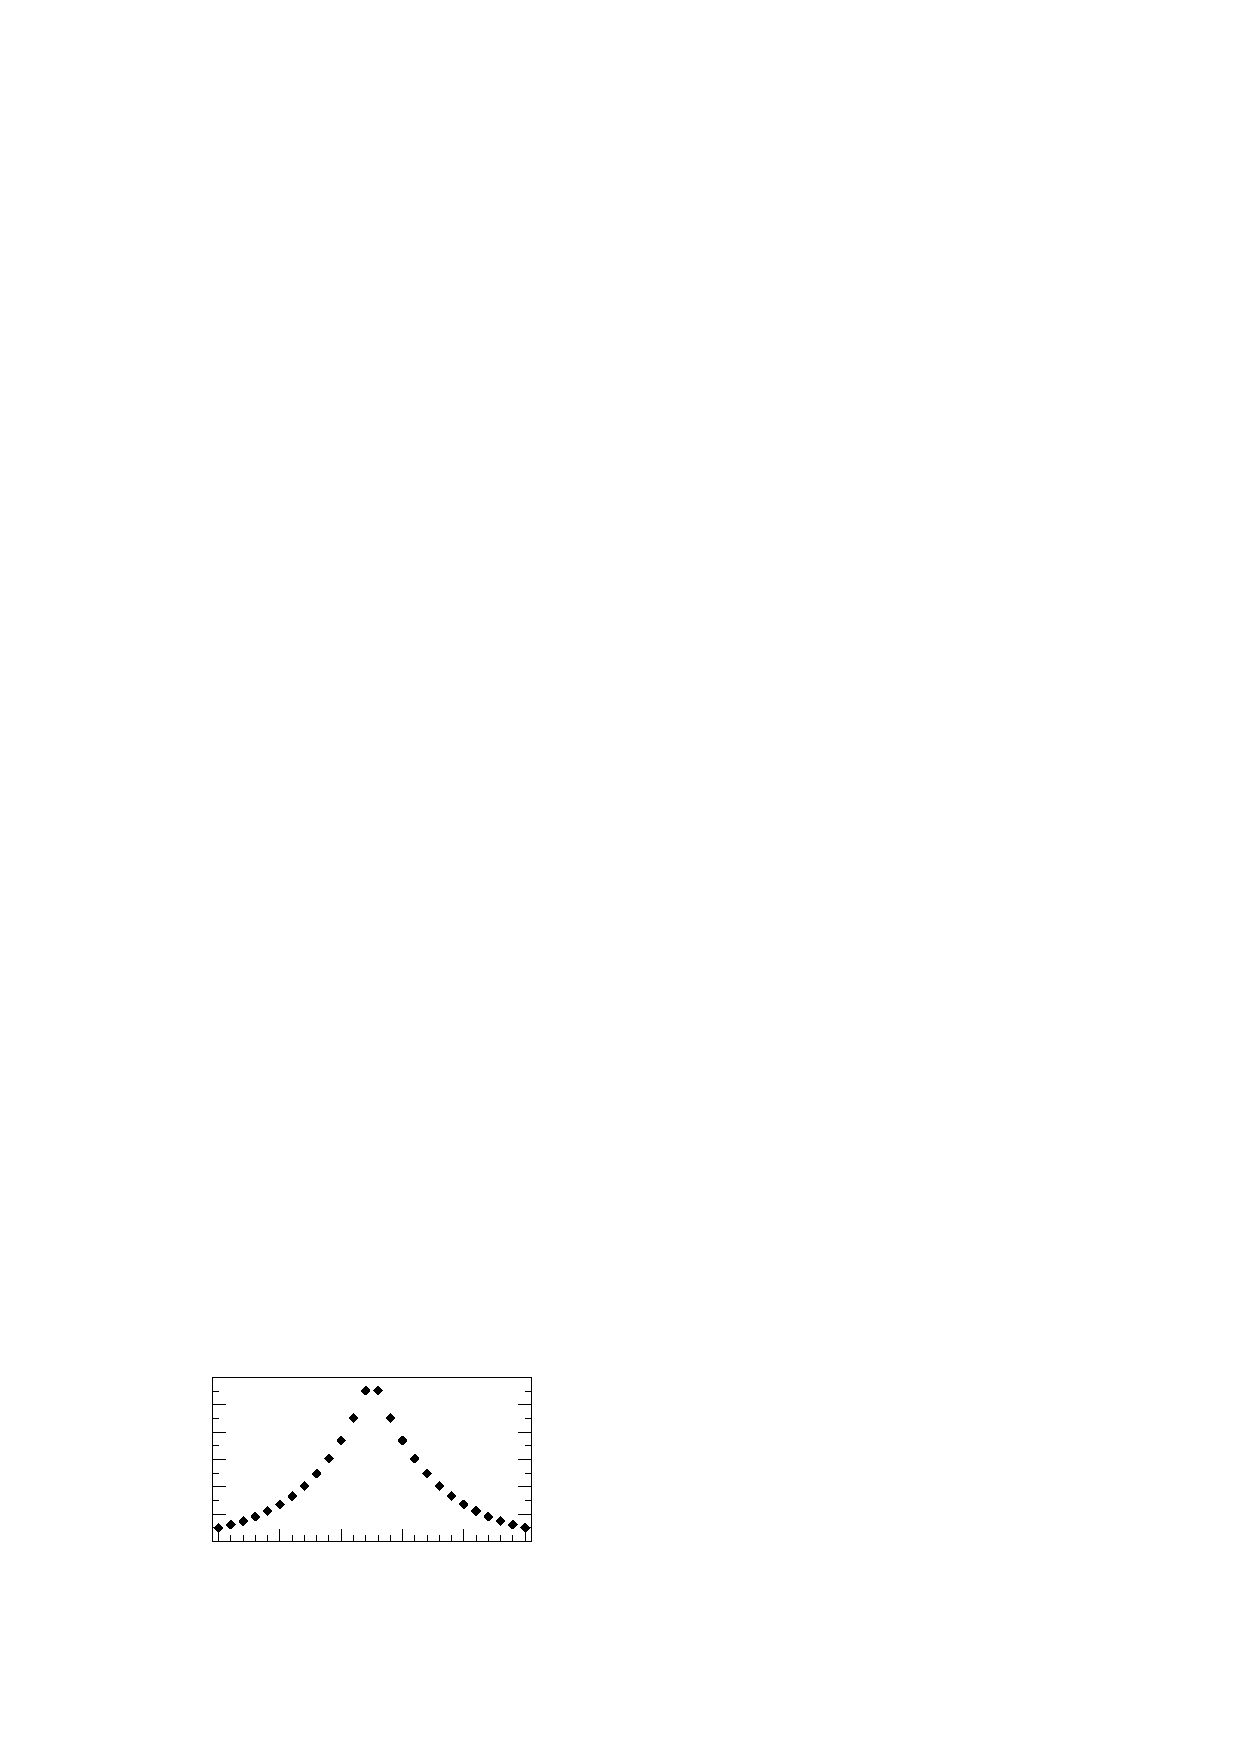
\includegraphics{position_weights}%
\end{picture}%
\begingroup
\setlength{\unitlength}{0.0200bp}%
\begin{picture}(9900,5940)(0,0)%
\put(1250,1500){\makebox(0,0)[r]{\strut{} 0}}%
\put(1250,2157){\makebox(0,0)[r]{\strut{} 2}}%
\put(1250,2813){\makebox(0,0)[r]{\strut{} 4}}%
\put(1250,3470){\makebox(0,0)[r]{\strut{} 6}}%
\put(1250,4127){\makebox(0,0)[r]{\strut{} 8}}%
\put(1250,4783){\makebox(0,0)[r]{\strut{} 10}}%
\put(1250,5440){\makebox(0,0)[r]{\strut{} 12}}%
\put(1647,1000){\makebox(0,0){\strut{} 0}}%
\put(3118,1000){\makebox(0,0){\strut{} 5}}%
\put(4589,1000){\makebox(0,0){\strut{} 10}}%
\put(6061,1000){\makebox(0,0){\strut{} 15}}%
\put(7532,1000){\makebox(0,0){\strut{} 20}}%
\put(9003,1000){\makebox(0,0){\strut{} 25}}%
%\put(5325,250){\makebox(0,0){\strut{}$b_{s,k}$}}%
\end{picture}%
\endgroup
\endinput

%%% Local Variables: 
%%% mode: latex
%%% TeX-master: t
%%% End: 
